\section{Descripción estructural de un multiplexor con \textit{IP Catalog} \label{sec:s2}}

\begin{center}
	\begin{minipage}{12cm}
		\begin{tcolorbox}[title=Actividad 2]
			Describir el multiplexor en forma estructural usando una función creada por el \textit{IP Catalog} siguiendo los pasos descritos en el documento o presentación. Simular el multiplexor.
		\end{tcolorbox}	
	\end{minipage}
\end{center}

La visualización RTL del circuito con múltiples asignaciones, descrito en Verilog, se muestra en la \autoref{fig:a_circuit3_rtl}. La implementación se hace con la instanciación de un multiplexor, denominado ``MyMux'', visualizado en el interior del módulo. Las simulaciones se visualizan en la \autoref{fig:a_circuit3_wave}, en donde se muestra que el multiplexor descrito opera de manera correcta.

En los Anexos se localiza la descripción en Verilog de este multiplexor. En el código se tienen dos módulos, siendo el primero, el de la jerarquía más alta y en donde se realiza la declaración de las entradas y la salida, para luego instanciar al módulo llamado ``MyMux'' con la etiqueta ``u0''. Cabe señalar que los argumentos de la instancia se deben colocar en el orden correcto. El segundo módulo unicamente es la descripción de un multiplexor sencillo, utilizando el operador condicional ``?''.

\begin{figure}[ht]
	\centering
	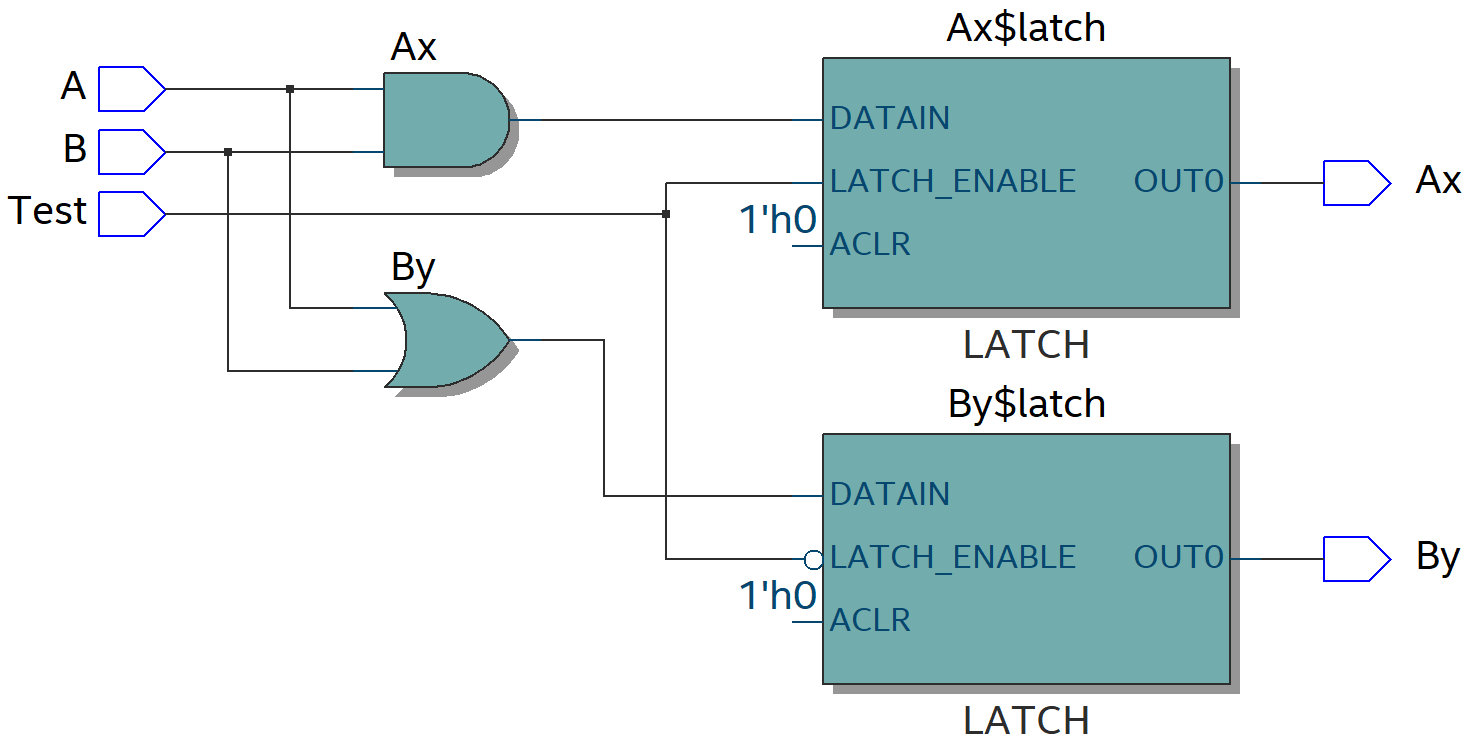
\includegraphics[scale=0.45]{Assignment_Circuit3_RTL.png}
	\caption{Diagrama RTL del circuito con múltiples asignaciones, descrito en Verilog. \label{fig:a_circuit3_rtl}}
\end{figure}

\begin{figure}[ht]
	\centering
	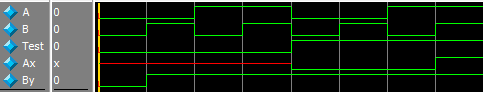
\includegraphics[scale=2]{Assignment_Circuit3_Wave.png}
	\caption{Simulación del circuito con múltiples asignaciones, descrito en Verilog, con el visor de formas de onda de ModelSim. \label{fig:a_circuit3_wave}}
\end{figure}